\chapter{Results}
%\thispagestyle{empty}

%\section{Experiments}

\section{Dictionary elements}

\begin{figure}[h]
\centering

\includegraphics[width = 0.33\textwidth]{images/gradient.png} 
\caption{gradient}
\label{fig:gradient}
\end{figure}

\begin{figure}[h]
\centering

\includegraphics[width = 0.33\textwidth]{images/checkerboard.png}
\caption{checkerboard}
\label{fig:checkerboard}
\end{figure}


\begin{figure}[h]
\centering

\includegraphics[width = 0.33\textwidth]{images/spot.png} 
\caption{spot}
\label{fig:spot}
\end{figure}


\begin{figure}[h]
\centering

\includegraphics[width = 0.33\textwidth]{images/edges.png}
\caption{edge}
\label{fig:edge}
\end{figure}

\begin{figure}[h]
\centering

\includegraphics[width = 0.33\textwidth]{images/wavelet.png}
\caption{wavelets}
\label{fig:wavelets}
\end{figure}

\section{Natural image database}

Convergence

% \begin{figure}[h]
% \centering
% 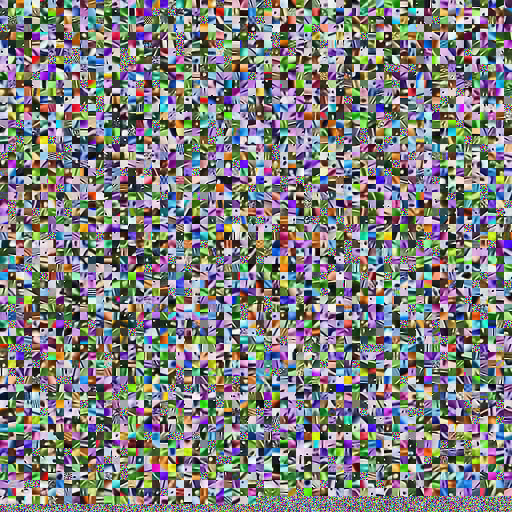
\includegraphics[width = 0.44\textwidth]{images/8_4000_10000_10_lasso.png} 
% \caption{8x8 OMP after some iterations}
% \label{fig:8_4000_lasso}
% \end{figure}
% 
% \begin{figure}[h]
% \centering
% 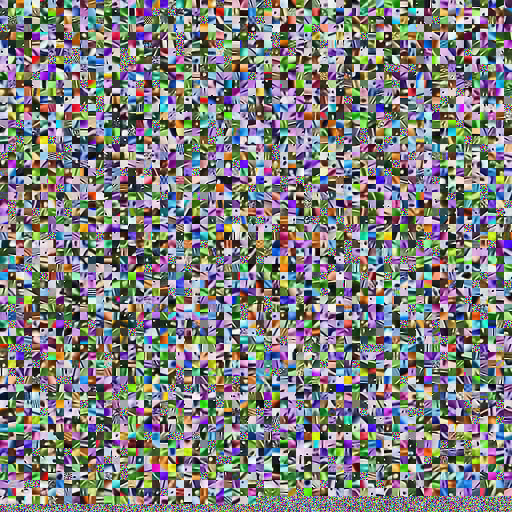
\includegraphics[width = 0.44\textwidth]{images/8_4000_10000_10_lasso.png} 
% \caption{8x8 LARS after some iterations}
% \label{fig:8_4000_lasso}
% \end{figure}

See the differences in the selection sceme.
In the beginning OMP is very random.

\begin{figure}[h]
\centering

\includegraphics[width = 0.66\textwidth]{images/1000_sketches.png}
\caption{1000 16x16 elements of sketches database}
\label{fig:16_1000_lasso}
\end{figure}

Mostly reduced to line segments and curve elements.
\Todo{Reconstruction results}

\begin{figure}[h]
\centering
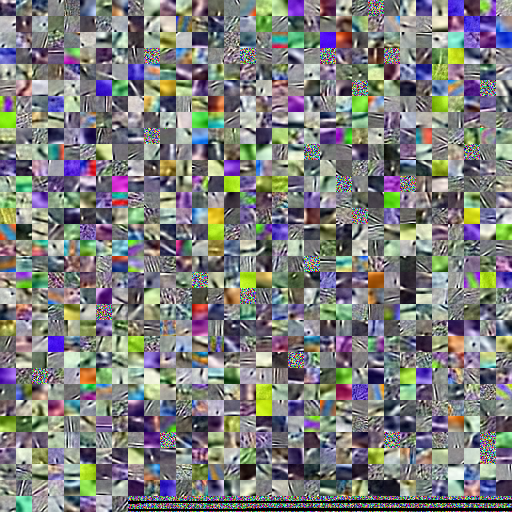
\includegraphics[width = 0.66\textwidth]{images/16_1000_1000_10_lasso.png}
\caption{8x8 elements of gogh}
\label{fig:16_1000_lasso}
\end{figure}

Similar to natural images.
compression dicts

\begin{figure}[h]
\centering
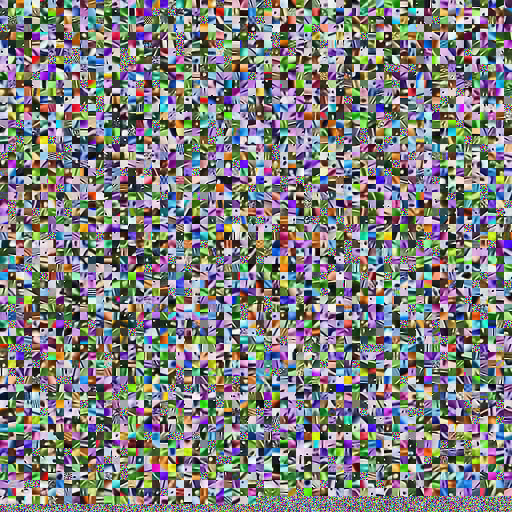
\includegraphics[width = 0.44\textwidth]{images/8_4000_10000_10_lasso.png} 
\caption{8x8 LARS-lasso with 4000 elements natural images}
\label{fig:8_4000_lasso}
\end{figure}

\Todo{Reconstruction results}

\begin{figure}[h]
\centering
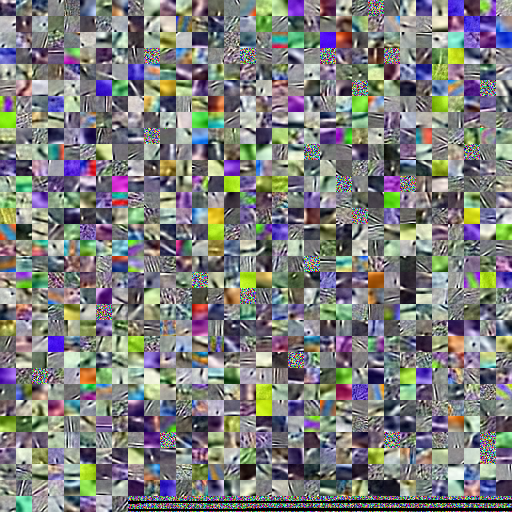
\includegraphics[width = 0.44\textwidth]{images/16_1000_1000_10_lasso.png}
\caption{16x16 LARS-lasso with 1000 elements}
\label{fig:16_1000_lasso}
\end{figure}

\Todo{Reconstruction results}

\begin{figure}
\centering
\subfloat[low pass]{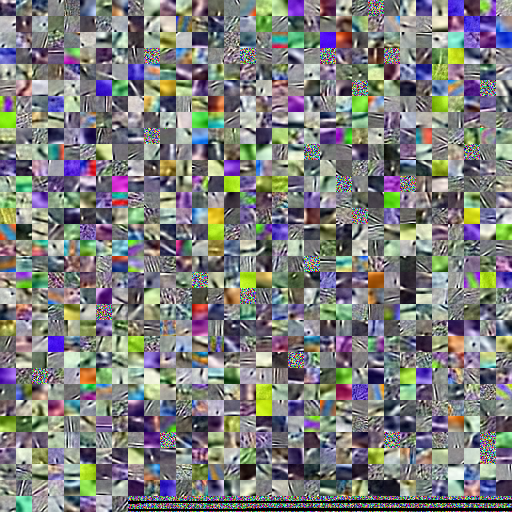
\includegraphics[width =
0.4\textwidth]{images/16_1000_1000_10_lasso.png}}
\hspace{5mm}
\subfloat[high pass]{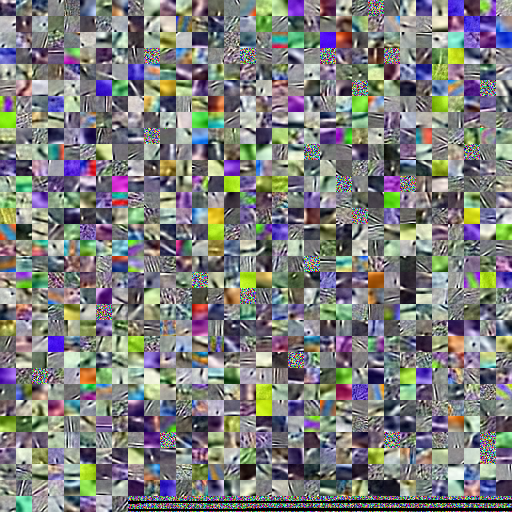
\includegraphics[width =
0.4\textwidth]{images/16_1000_1000_10_lasso.png}}
\caption{low pass}
\label{fig:16_1000_lasso}
\end{figure}


\Todo{Reconstruction results}


\section{Specific image groups}


\section{Compression}

%\section{Quality}
%\subsection*{trained vs. analytical base}
%\subsection*{Compression ratio}
%\subsection*{Dictionary size}
%Setup:
%  initialize: random pixels, radom samples 
%  dict size: 256, 1000, 4000, 8000
%  coeffs: 5, 10, 20









